%%% Titulní strana práce a další povinné informační strany

%%% Titulní strana práce

\pagestyle{empty}
\pagenumbering{gobble}
\hypersetup{pageanchor=false}

\begin{center}
\LARGE
\textbf{GYMNASIUM JANA KEPLERA}\\
{\large Parléřova 2/118, 169 00 Praha 6}

\vspace{\stretch{3}}


\includegraphics[width=.3\textwidth]{img/logo}

\vspace{\stretch{3}}

{\Huge\bfseries\NazevPrace}

\vspace{8mm}
\mdseries{Maturitní práce}

\vspace{\stretch{8}}
\large
\begin{tabular}{rl}
Autor: & \AutorPrace \\
\noalign{\vspace{2mm}}
Třída: & \Trida\\
\noalign{\vspace{2mm}}
Školní rok: & 2023/2024\\
\noalign{\vspace{2mm}}
Předmět: & Informatika \\
\noalign{\vspace{2mm}}
Vedoucí práce: & \Vedouci \\
\end{tabular}

\vspace{20mm}
Praha, \DatumOdevzdani
\end{center}


\openright

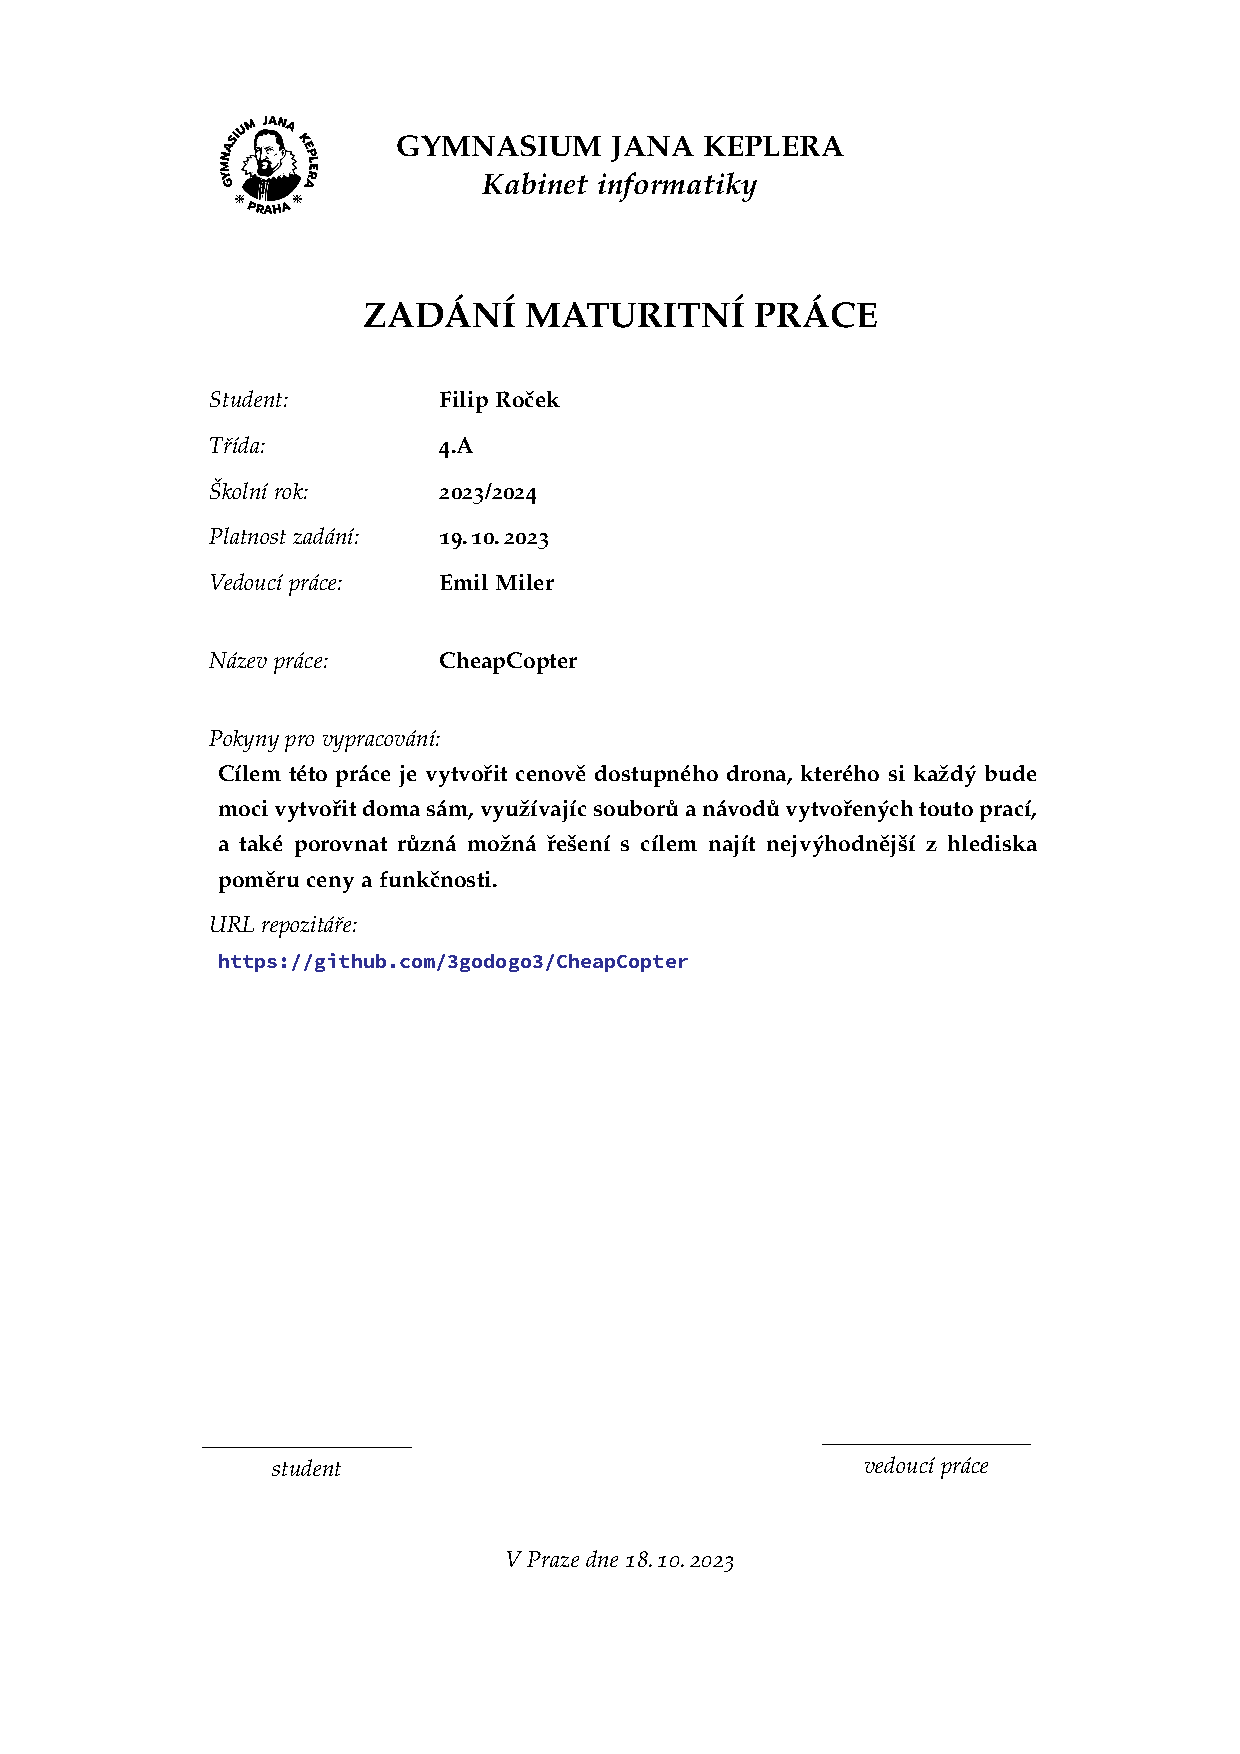
\includepdf[]{zadani.pdf}


%%% Strana s čestným prohlášením k bakalářské práci

\hypersetup{pageanchor=true}
\cleardoublepage
\vspace*{\fill}
\section*{Prohlášení}
\noindent
\Prohlaseni

\vspace{2cm}
\noindent
V Praze dne \today
\hspace*{\fill}\small{\AutorPrace}
\vspace{1cm}

%%% Povinná informační strana bakalářské práce
\openright
\section*{Abstrakt}
\noindent
\Abstrakt

\openright
\pagenumbering{arabic}